% Activate the following line by filling in the right side. If for example the name of the root file is Main.tex, write
% "...root = Main.tex" if the chapter file is in the same directory, and "...root = ../Main.tex" if the chapter is in a subdirectory.
 
%!TEX root =  dissertation.tex

\chapter[Analysis]{Analysis}

\section{Usability result and analysis}

\subsection{Demography}


\vspace{1cm}

\noindent%
\begin{minipage}{\linewidth}% to keep image and caption on one page
\makebox[\linewidth]{
  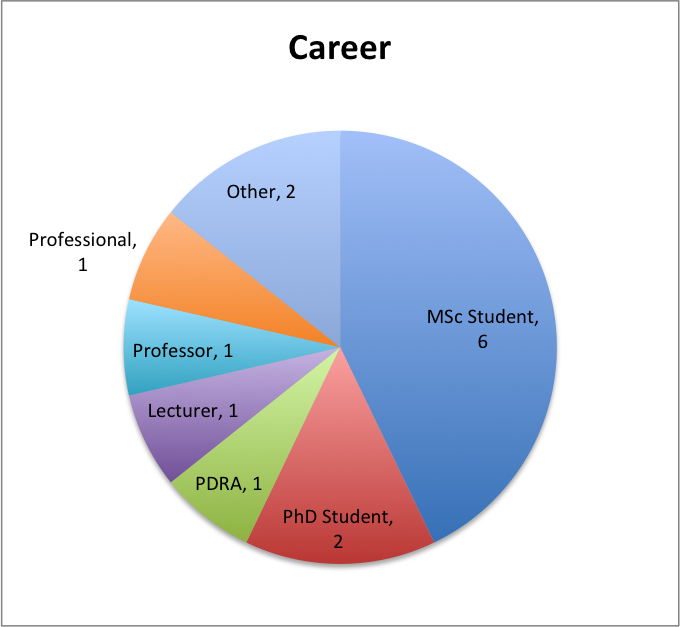
\includegraphics[keepaspectratio=true,scale=0.6]{../resources/evaluation/usability/career.png}
 }
\captionof{figure}{Career distribution} \label{fig:survey-career}%      only if needed  
\end{minipage}

\vspace{1cm}

\vspace{1cm}

\noindent%
\begin{minipage}{\linewidth}% to keep image and caption on one page
\makebox[\linewidth]{
  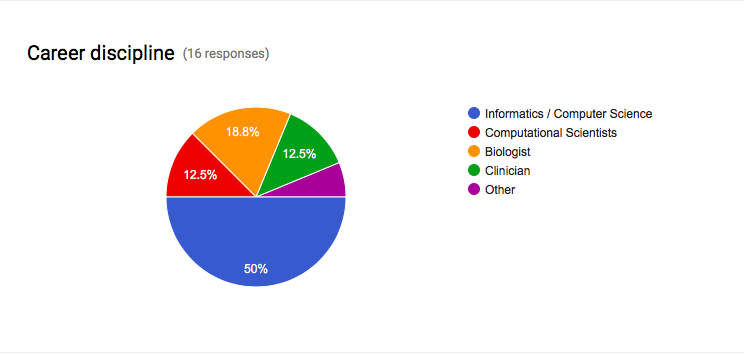
\includegraphics[keepaspectratio=true,scale=0.6]{../resources/evaluation/usability/discipline.png}
 }
\captionof{figure}{Career discipline} \label{fig:survey-discipline}%      only if needed  
\end{minipage}

\vspace{1cm}

\noindent%
\begin{minipage}{\linewidth}% to keep image and caption on one page
\makebox[\linewidth]{
  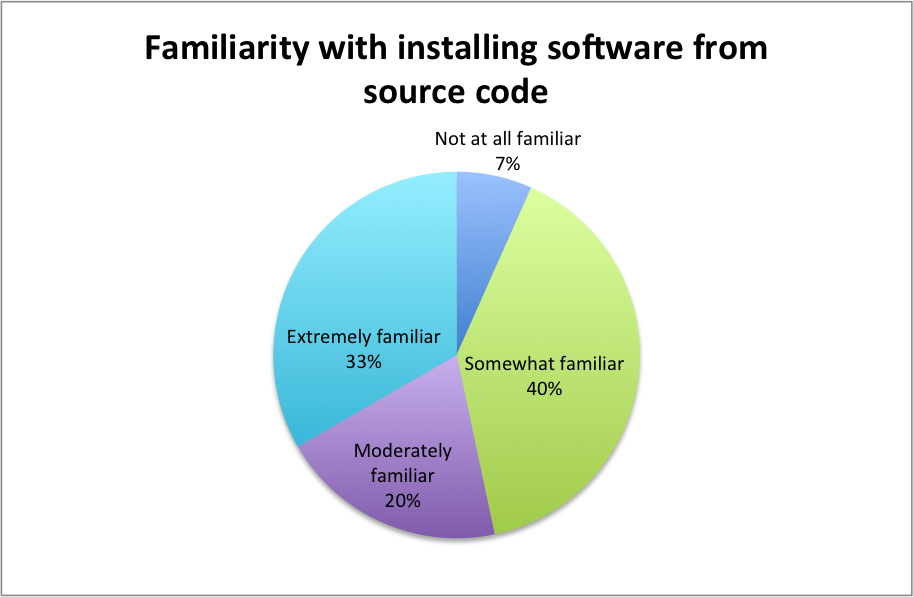
\includegraphics[keepaspectratio=true,scale=0.8]{../resources/evaluation/usability/source_code.png}
 }
\captionof{figure}{Familiarity with installing software from source code} \label{fig:survey-source}%      only if needed  
\end{minipage}

\vspace{1cm}

\noindent%
\begin{minipage}{\linewidth}% to keep image and caption on one page
\makebox[\linewidth]{
  
\includegraphics[keepaspectratio=true,scale=0.8]{../resources/evaluation/usability/browser.png}
 }
\captionof{figure}{Familiarity with web browser} \label{fig:survey-browser}%      only if needed  
\end{minipage}

\vspace{1cm}

\noindent%
\begin{minipage}{\linewidth}% to keep image and caption on one page
\makebox[\linewidth]{
  
\includegraphics[keepaspectratio=true,scale=0.8]{../resources/evaluation/usability/browser.png}
 }
\captionof{figure}{Familiarity with CFD tools like HemeLB} \label{fig:survey-hemelb}%      only if needed  
\end{minipage}

\vspace{1cm}



\subsection{Scenario 1: Run a simulation}

\vspace{1cm}

\noindent%
\begin{minipage}{\linewidth}% to keep image and caption on one page
\makebox[\linewidth]{
  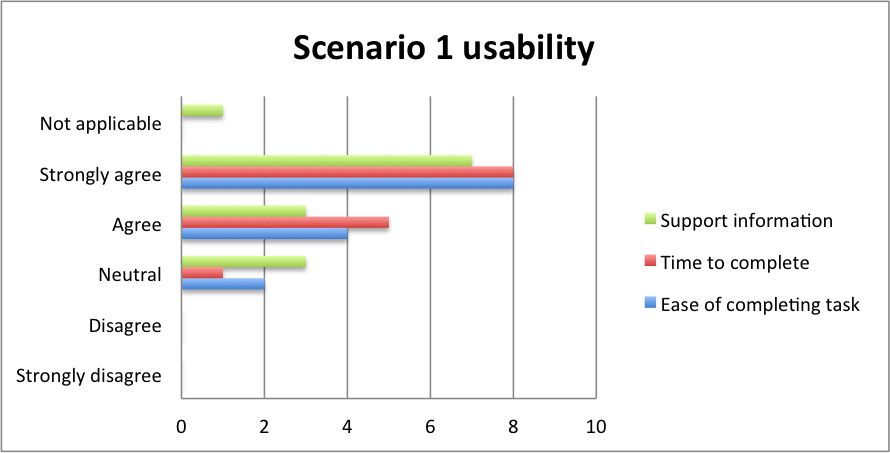
\includegraphics[keepaspectratio=true,scale=0.9]{../resources/evaluation/usability/scenario1_usability.png}
 }
\captionof{figure}{Scenario 1 usability} \label{fig:survey-s1-usability}%      only if needed  
\end{minipage}

\vspace{1cm}

\noindent%
\begin{minipage}{\linewidth}% to keep image and caption on one page
\makebox[\linewidth]{
  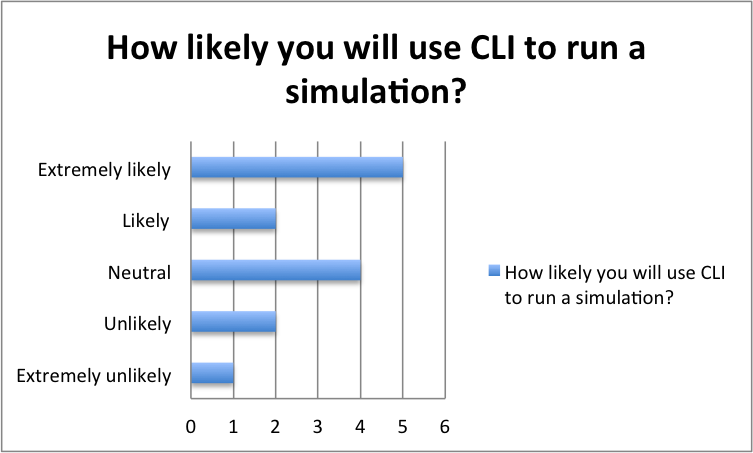
\includegraphics[keepaspectratio=true,scale=0.9]{../resources/evaluation/usability/scenario1_cli.png}
 }
\captionof{figure}{Scenario 1 command line preference} \label{fig:survey-s1-cli}%      only if needed  
\end{minipage}

\vspace{1cm}

\noindent%
\begin{minipage}{\linewidth}% to keep image and caption on one page
\makebox[\linewidth]{
  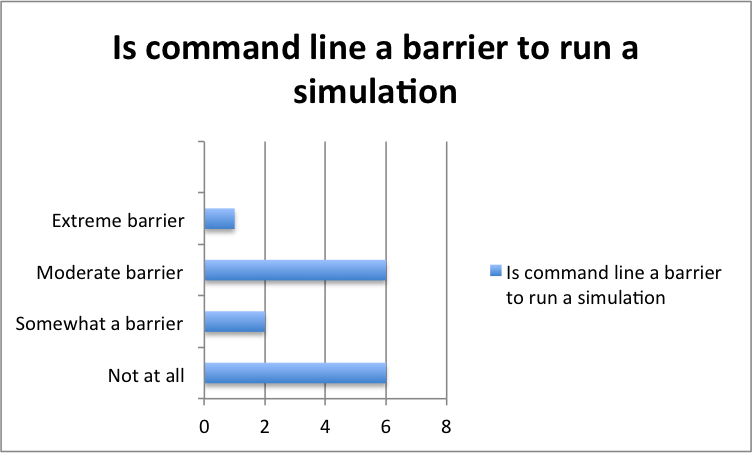
\includegraphics[keepaspectratio=true,scale=0.9]{../resources/evaluation/usability/scenario1_cli_barrier.png}
 }
\captionof{figure}{Scenario 1 barrier in using command line} \label{fig:survey-s1-cli-barrier}%      only if needed  
\end{minipage}

\vspace{1cm}



\subsection{Scenario 2: Reproduce past simulation}

\vspace{1cm}

\noindent%
\begin{minipage}{\linewidth}% to keep image and caption on one page
\makebox[\linewidth]{
  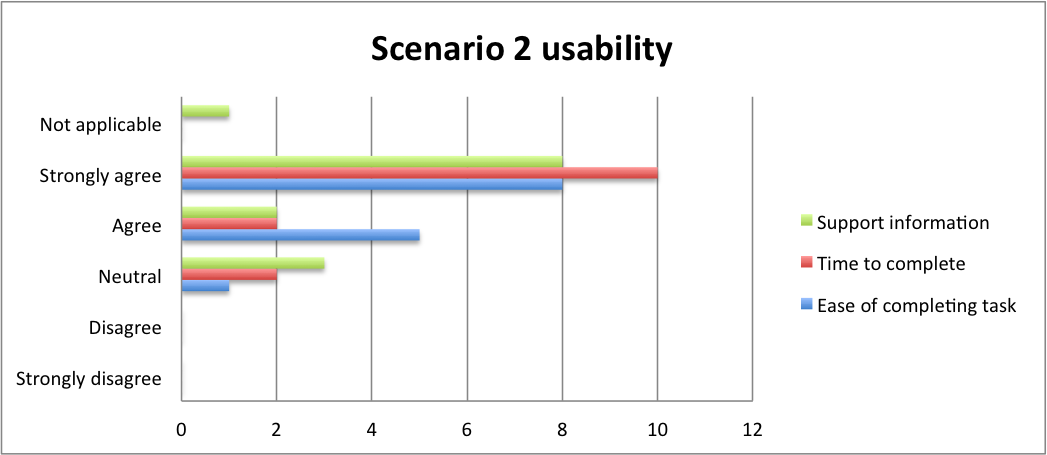
\includegraphics[keepaspectratio=true,scale=0.9]{../resources/evaluation/usability/scenario2_usability.png}
 }
\captionof{figure}{Scenario 2 usability} \label{fig:survey-s2-usability}%      only if needed  
\end{minipage}

\vspace{1cm}

\noindent%
\begin{minipage}{\linewidth}% to keep image and caption on one page
\makebox[\linewidth]{
  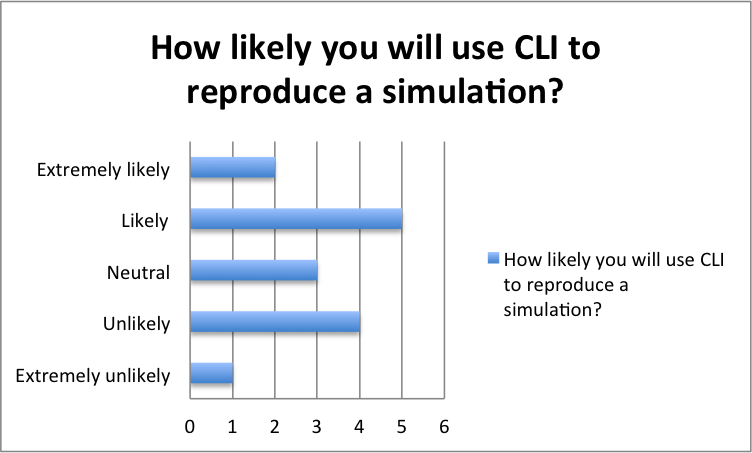
\includegraphics[keepaspectratio=true,scale=0.9]{../resources/evaluation/usability/scenario2_cli.png}
 }
\captionof{figure}{Scenario 2 command line preference} \label{fig:survey-s2-cli}%      only if needed  
\end{minipage}

\vspace{1cm}

\noindent%
\begin{minipage}{\linewidth}% to keep image and caption on one page
\makebox[\linewidth]{
  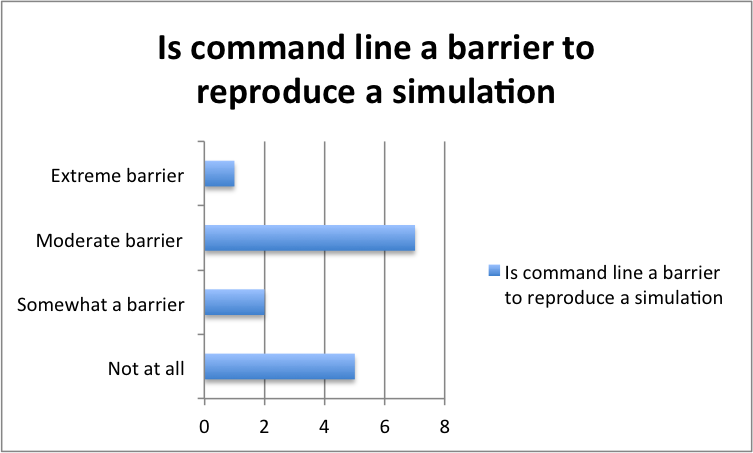
\includegraphics[keepaspectratio=true,scale=0.9]{../resources/evaluation/usability/scenario2_cli_barrier.png}
 }
\captionof{figure}{Scenario 2 barrier in using command line} \label{fig:survey-s2-cli-barrier}%      only if needed  
\end{minipage}

\vspace{1cm}



\subsection{Overall usability}


%%%%%%%%%%%%%%%%%%%%%%%%%%%%%%%%%%%
%  SYSTEM USEFULNESS 
%%%%%%%%%%%%%%%%%%%%%%%%%%%%%%%%%%%
\begin{center}
\captionof{table}{System usefulness}\label{table:overall-usability}
\scalebox{0.75}{

\begin{tabular}{|l|l|l|l|l|l|l|}
\hline
                                                            & \begin{tabular}[c]{@{}l@{}}Strongly\\  disagree\end{tabular} & Disagree & Neutral & Agree & \begin{tabular}[c]{@{}l@{}}Strongly\\  agree\end{tabular} & \begin{tabular}[c]{@{}l@{}}Not \\ applicable\end{tabular} \\ \hline
how easy it is to use this system                           & 0                                                            & 0        & 0       & 8     & 7                                                         & 0                                                         \\ \hline
It was simple to use this system                            & 0                                                            & 0        & 0       & 2     & 13                                                        & 0                                                         \\ \hline
I can effectively complete my work using this system        & 1                                                            & 1        & 2       & 3     & 4                                                         & 4                                                         \\ \hline
I am able to complete my work quickly using this system     & 0                                                            & 1        & 3       & 3     & 6                                                         & 2                                                         \\ \hline
I am able to efficiently complete my work using this system & 0                                                            & 2        & 2       & 4     & 5                                                         & 2                                                         \\ \hline
I feel comfortable using this system                        & 1                                                            & 1        & 0       & 3     & 10                                                        & 0                                                         \\ \hline
It was easy to learn to use this system                     & 0                                                            & 0        & 2       & 0     & 13                                                        & 0                                                         \\ \hline
I believe I became productive quickly using this system     & 0                                                            & 1        & 2       & 3     & 5                                                         & 4                                                         \\ \hline
\end{tabular}
}
\end{center}
\vspace{1cm}


%%%%%%%%%%%%%%%%%%%%%%%%%%%%%%%%%%%
%  INFO QUALITY
%%%%%%%%%%%%%%%%%%%%%%%%%%%%%%%%%%%

\begin{center}
\captionof{table}{Information quality}\label{table:overall-info-quality}
\scalebox{0.75}{
\begin{tabular}{|l|l|l|l|l|l|l|}
\hline
                                                                                                                                                                               & \begin{tabular}[c]{@{}l@{}}Strongly\\ disagree\end{tabular} & Disagree & Neutral & Agree & \begin{tabular}[c]{@{}l@{}}Strongly\\ agree\end{tabular} & \begin{tabular}[c]{@{}l@{}}Not\\ applicable\end{tabular} \\ \hline
\begin{tabular}[c]{@{}l@{}}The system gives error messages that\\  clearly tell me how to fix problems\end{tabular}                                                            & 0                                                           & 2        & 1       & 4     & 2                                                        & 6                                                        \\ \hline
\begin{tabular}[c]{@{}l@{}}Whenever I make a mistake using the system, \\ I recover easily and quickly\end{tabular}                                                            & 0                                                           & 0        & 5       & 1     & 3                                                        & 6                                                        \\ \hline
\begin{tabular}[c]{@{}l@{}}The information (such as online help, \\ on-screen messages, and other documentation)\\  provided with this system is clear\end{tabular}            & 0                                                           & 0        & 3       & 4     & 5                                                        & 3                                                        \\ \hline
It is easy to find the information I needed                                                                                                                                    & 0                                                           & 1        & 2       & 3     & 6                                                        & 3                                                        \\ \hline
\begin{tabular}[c]{@{}l@{}}The information (such as online help,\\  on-screen messages, and other documentation)\\  provided for the system is easy to understand\end{tabular} & 0                                                           & 1        & 2       & 5     & 6                                                        & 1                                                        \\ \hline
\begin{tabular}[c]{@{}l@{}}The information is effective in helping me\\  complete the tasks and scenarios\end{tabular}                                                         & 0                                                           & 1        & 4       & 2     & 7                                                        & 1                                                        \\ \hline
\begin{tabular}[c]{@{}l@{}}The organization of information on the \\ system screens is clear\end{tabular}                                                                      & 0                                                           & 0        & 3       & 8     & 4                                                        & 0                                                        \\ \hline
\end{tabular}

}
\end{center}
\vspace{1cm}



%%%%%%%%%%%%%%%%%%%%%%%%%%%%%%%%%%%
%  INTERFACE QUALITY
%%%%%%%%%%%%%%%%%%%%%%%%%%%%%%%%%%%
\begin{center}
\captionof{table}{Interface quality}\label{table:overall-interface-quality}
\scalebox{0.75}{
\begin{tabular}{|l|l|l|l|l|l|l|}
\hline
                                                                                                                  & \begin{tabular}[c]{@{}l@{}}Strongly\\ disagree\end{tabular} & Disagree & Neutral & Agree & \begin{tabular}[c]{@{}l@{}}Strongly\\ agree\end{tabular} & \begin{tabular}[c]{@{}l@{}}Not\\ applicable\end{tabular} \\ \hline
The interface of this system is pleasant                                                                          & 1                                                           & 1        & 1       & 7     & 5                                                        & 0                                                        \\ \hline
I like using the interface of this system                                                                         & 0                                                           & 2        & 1       & 8     & 4                                                        & 0                                                        \\ \hline
\begin{tabular}[c]{@{}l@{}}This system has all the functions and\\  capabilities I expect it to have\end{tabular} & 1                                                           & 2        & 1       & 4     & 4                                                        & 3                                                        \\ \hline
Overall, I am satisfied with this system                                                                          & 0                                                           & 0        & 2       & 7     & 6                                                        & 0                                                        \\ \hline
\end{tabular}
}
\end{center}
\vspace{1cm}

\section{Performance result and analysis}

In this section, I will discuss the performance benchmark of HemeLB simulation done in ARCHER supercomputer, Indy2 HPC cluster, and AWS EC2 where HemeWeb is deployed to. HemeLB produced a report files that can be used to benchmark the performance of the simulation execution. I made sure that on each infrastructure, the input file we used is the same. I took the simulation total time result from that files and compare the value between infrastructure.


\begin{center}

\captionof{table}{Performance comparison HemeLB on Indy2 vs AWS EC2}\label{table:perf}

\begin{tabular}{|c|c|c|}
\hline
\multicolumn{1}{|l|}{}            & \multicolumn{2}{c|}{Performance in seconds}               \\ \hline
\multicolumn{1}{|c|}{\# of Cores} & \multicolumn{1}{c|}{Indy2} & \multicolumn{1}{c|}{AWS EC2} \\ \hline
36                                & 24.7                       & 36.3                         \\ \hline
72                                & 12.7                       & 29.9                         \\ \hline
144                               & 7.08                       & 36.5                         \\ \hline
288                               & 3.44                       & 32.4                         \\ \hline
576                               & 1.81                       & 20.4                         \\ \hline
1152                              & 1.58                       & N/A                             \\ \hline
\end{tabular}

\end{center}



\vspace{1cm}

\begin{center}
\captionof{table}{HemeLB performance on ARCHER supercomputer}\label{table:perf-archer}
\begin{tabular}{|c|c|c|}
\hline
\multicolumn{1}{|l|}{}            & \multicolumn{1}{c|}{Performance in seconds}               \\ \hline
\multicolumn{1}{|l|}{\# of Cores} & \multicolumn{1}{c|}{ARCHER}  \\ \hline
24                                & 24.7                                           \\ \hline
48                                & 12.7                                         \\ \hline
96                               & 7.08                                       \\ \hline
192                               & 3.44                                           \\ \hline
384                               & 1.81                                               \\ \hline
768                              & 1.58                                              \\ \hline
1536                              & 1.58                                              \\ \hline
\end{tabular}
\end{center}


\vspace{1cm}

\noindent%
\begin{minipage}{\linewidth}% to keep image and caption on one page
\makebox[\linewidth]{
  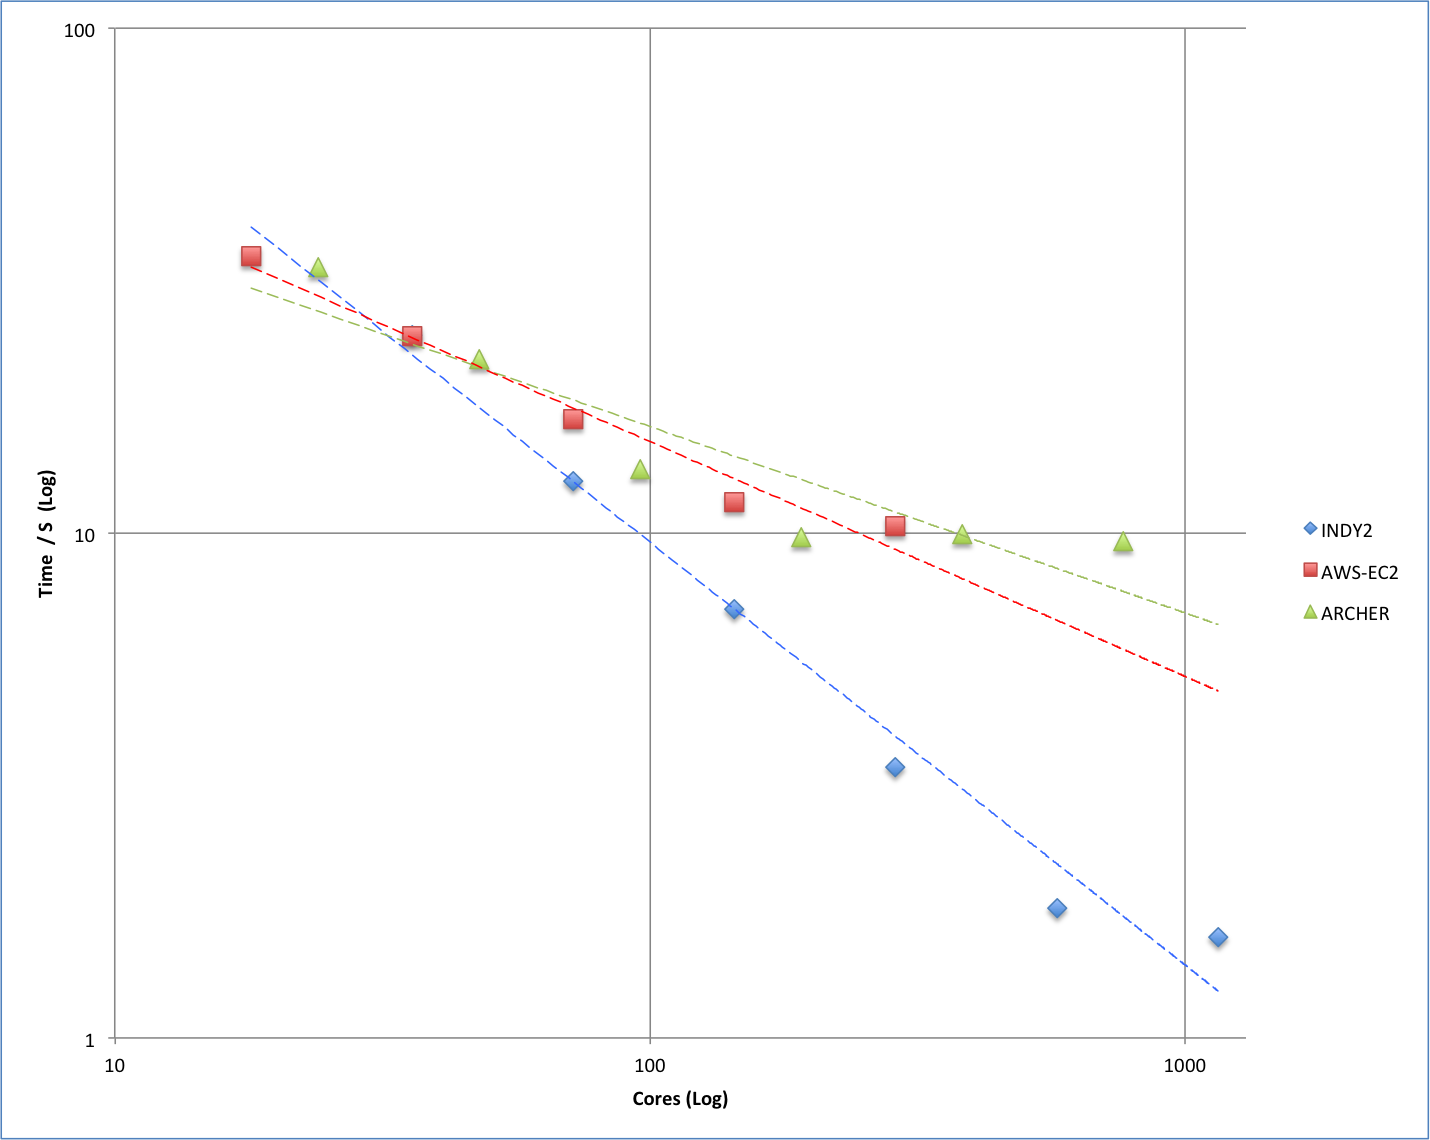
\includegraphics[keepaspectratio=true,scale=0.75]{../resources/evaluation/performance/overview.png}
 }
\captionof{figure}{HemeLB performance comparison} \label{fig:hemelb-perf-overview}%      only if needed  
\end{minipage}

\vspace{1cm}


In general, the performance of HemeLB with cloud infrastructure is worse when compared to ARCHER and Indy2. On each simulation instances with a different number of cores, we see slower simulation execution result when compared to the likes of the Indy2 machine and ARCHER supercomputer as observed on table \ref{table:perf}, \ref{table:perf-archer} and figure \ref{fig:hemelb-perf-overview}.

ARCHER supercomputer has slower simulation time compared to Indy2, because of the difference of processors used in the compute node. ARCHER used a three-year-old 2.7 GHz, 12-core E5-2697 v2 Ivy Bridge processor. Compared to Indy2 which boasts the newer Broadwell-based Intel(R) Xeon(R) CPU E5-2695 v4 @ 2.10GHz. The number of thread inside those processors also differ, ARCHER has 24 while Indy2 has 36. This makes the performance difference. On the other hand for this evaluation, we use Amazon's c4.8xlarge EC2 instance which has Haswell-based E5-2666 v3 processor that has 36 virtual CPU cores. All these difference contributes toward the speed difference oh the simulation results.

The scaling of the performance is where HemeWeb took a dive. It is apparent that with increased compute node, the network activity between the nodes become a bottleneck in the HemeWeb's case. The performance dip when we started the simulation using 4 compute nodes which have 144 cores that it is slower than just using 1 compute node. However, the performance improves as we add more compute nodes. This is not seen in the case of Indy2, where it scales very well and reach a diminishing return on the performance after using more than 1,000 cores.